% !TEX root = ../Thesis.tex
\chapter{Evaluation}
\label{c:evaluation}

This chapter is separated into two sections. The first section aims to validate and verify the implementation in terms of their
correct execution. It focuses on the core contributions, such as the lazy replicaiton algorithm as well as the freshness filter capability.
Further it ensures the correct handling of the described constraints and establishes certain test cases to identify possibile failures that can occur 
during execution as well as suitable failure handling scenarios.

The second part of this chapter focuses on benchmarking the implementation on the basis of the described motivational scenario itself.
Since one of the main goals was to relax the consistency and allow 
This is followed by comparing the performance of several cases to identify how the system will behave in certain situations.
Further it will compare several executions to determine how the impleemntation affect the providede requirements.

Furthermore the performance of the individual functionalities is benchmarked and compared against slightly adjusted variations 
to give an comprehensive overview of the impact.


\section{Goal}
The evaluation has two goals the correctness as well as the impact of data freshness onto different kinds of workloads.

Verify and validate the correctness as well as the completeness of the implementation based on several characteristics.
These include the correct execution of lazy replication, the possibility to refresh statements on demand.

Impact of the replication engine on the underlying performance, if freshness indeed increases the overall parallel writes on the system.
Or if it is just marginally lower than before. Also compare this to the overall introduced overhead. And if the change was wort it



Compare underlying stores to assess the deviations of the polystore in total.
%%%%%%%%%%%%%%%%%%%%%%%%%%%%%%%%%%%%%%%%%%%%%%%%%%%%%%%%%%%%%%%%%%

\section{Correctness}

The correctness of the introduced solution mainly focuses on two parts. For one the replication behaviour, to verify if each lazy replication is carried out correctly,
and if not verify that reasonable counter measures are in place and apply them. This is crucial since we do not compare the footprint or the integrity of the data after 
a replication update. Rather we compare on a high level the metadata 
(i.e. if the number of modifications and the commit timestamp after the data replication are equal on primary and secondary node) of two replicas. 

The second part of the validation process focuses on the retrieval of outdated nodes. Although we always have a fall back to the primary placements as described in section \ref{sec:freshness_selection},
we still want to avoid excessive locking to parallelize requests to ultimately speed up the average response time.


\todo{Also checks for freshness specification if this can for one be even applied to the system , due to ongoing constraints or if it is even posssible to specify a freshness index >1.0}
\todoMissing{\ref{sec:constraints, lazy -> eager and outdated -> refreshable}}
\todoMissing{As already suggested within constrianst we have to ensure that data will not be lost}

\todoMissing{How to ensure that cached freshness objects are not falesely executed and secertly violating the specified freshness (It is rechecked)}

%%%%%%%%%%%%%%%%%%%%%%%%%%%%%%%%%%%%%%%%%%%%%%%%%%%%%%%%%%%%%%%%%%

\section{Benchmarks}

\todoMissing{Contain overhead as much as possible otherwise the freshness eveluation will negativiely impact regular operations}

\todo{Explain why it is necessary to verify the solution with different combinations}

\subsection{Evaluation Environment}
\todo{Elaborate and thoroughly explain why the environment was chosen and how the test was executed for the sake of rerpoducibility}


\subsection{Evaluation Procedure}
The following steps outline the procedure for benchmarking data freshness within Polypheny-DB.

\todo{Check how fast the replication is compared to the primary execution. Benchmark on two equal stores and measure the time}

\todo{ Execute benchmarks on multimodal dbs. as well as different kind of }

\todo{ Talk about implementation of freshness characteristic in many query languages}

\todoMissing{Check if freshness could even be used, or if we would always fallback to primary or when is the turining point when the freshness now works.}

\todoMissing{Using 3 Node and 5 Node with eager replication than the same using lazy replication without any freshneess queries.}

\todoMissing{Locking switched from table-wise to partition-wise. Compare unpartitioned table to horiontally partitioned table, single placment vs. distributed across stores}

\todoMissing{Convergence time on different stores and in general}

\todoMissing{Compare different evaluation types with each other, timestamp, absolute delay, relative delay and index mdoficiaiton and time}

\todoMissing{Schuldt FAS Evaluation possibilities}

\todoMissing{Also number of nodes-stores will have impact on query times replication time etc.}

\todoMissing{Execute on two stores, one time store is eager second tiem store 1 is lazy. Show how a mixed workload impacts the total processing time of a fixed benchmark }

\todoMissing{Story - konzept nicht Abstrakt und warum mit Polystore gut - mit Motivation verknüpfen}


\subsubsection{Compare Overhead} 
To see if the implementation has any impact on the genral processing time. 
Since every request through a polystore will impact the entire throughput, minimizing additonal overhead is crucial.
FIgure \ref{fig:overhead}
\begin{figure}[t] 
    \centering 
    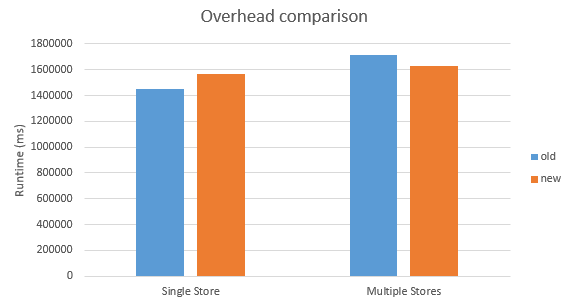
\includegraphics[width=0.7\textwidth]{Figures/overhead.png}
    \caption{Overhead comparison of the entire implemation.}
    \label{fig:overhead}
\end{figure}

%%%%%%%%%%%%%%%%%%%%%%%%%%%%%%%%%%%%%%%%%%%%%%%%%%%%%%%%%%%%%%%%%%

\subsubsection{Locking } 

Impact on locking adaptation. Comparing old locking model against the new locking model targeting partitions instead of entire table entities.

Comparing un partitioned vs. partitioned on a single and on nstores where n is the numbe rof partitions
figure \ref{fig:lock_comp} \ref{fig:oldlock} \ref{fig:newlock} \ref{fig:oldandnewlock}

\begin{figure}
    \centering
    \begin{subfigure}{.7\textwidth}
      \centering
      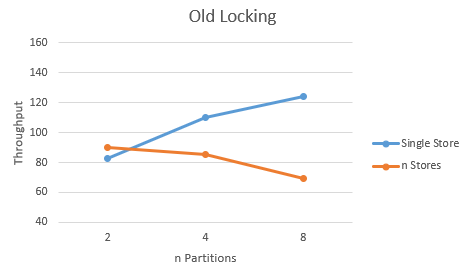
\includegraphics[width=.5\linewidth]{Figures/old_locking.PNG}
      \caption{A subfigure}
      \label{fig:oldlock}
    \end{subfigure}%
    \begin{subfigure}{.5\textwidth}
      \centering
      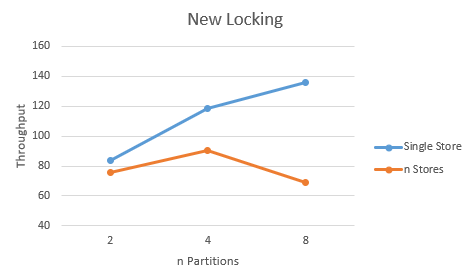
\includegraphics[width=.7\linewidth]{Figures/new_locking.PNG}
      \caption{A subfigure}
      \label{fig:newlock}
    \end{subfigure}
    \begin{subfigure}{.7\textwidth}
        \centering
        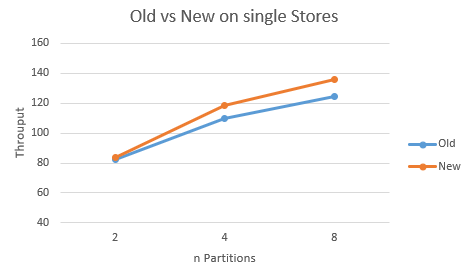
\includegraphics[width=.7\linewidth]{Figures/old_vs_new.PNG}
        \caption{Old vs. New}
        \label{fig:oldandnewlock}
      \end{subfigure}
    \caption{A figure with three subfigures}
    \label{fig:lock_comp}
\end{figure}




%%%%%%%%%%%%%%%%%%%%%%%%%%%%%%%%%%%%%%%%%%%%%%%%%%%%%%%%%%%%%%%%%%


\subsubsection{ Single PSQL vs HSQL } 

Ellaborate why DML only

First show single Performance on the Store to see which one is the slower one of these stores in our setup.
This will also show which stores logically bound the primary transaction time. PSQL on Docker. Since Docker Containers use a limited shared set of resources 
this store immitating a slower performinh node in oru setup.

\begin{figure}[t] 
    \centering 
    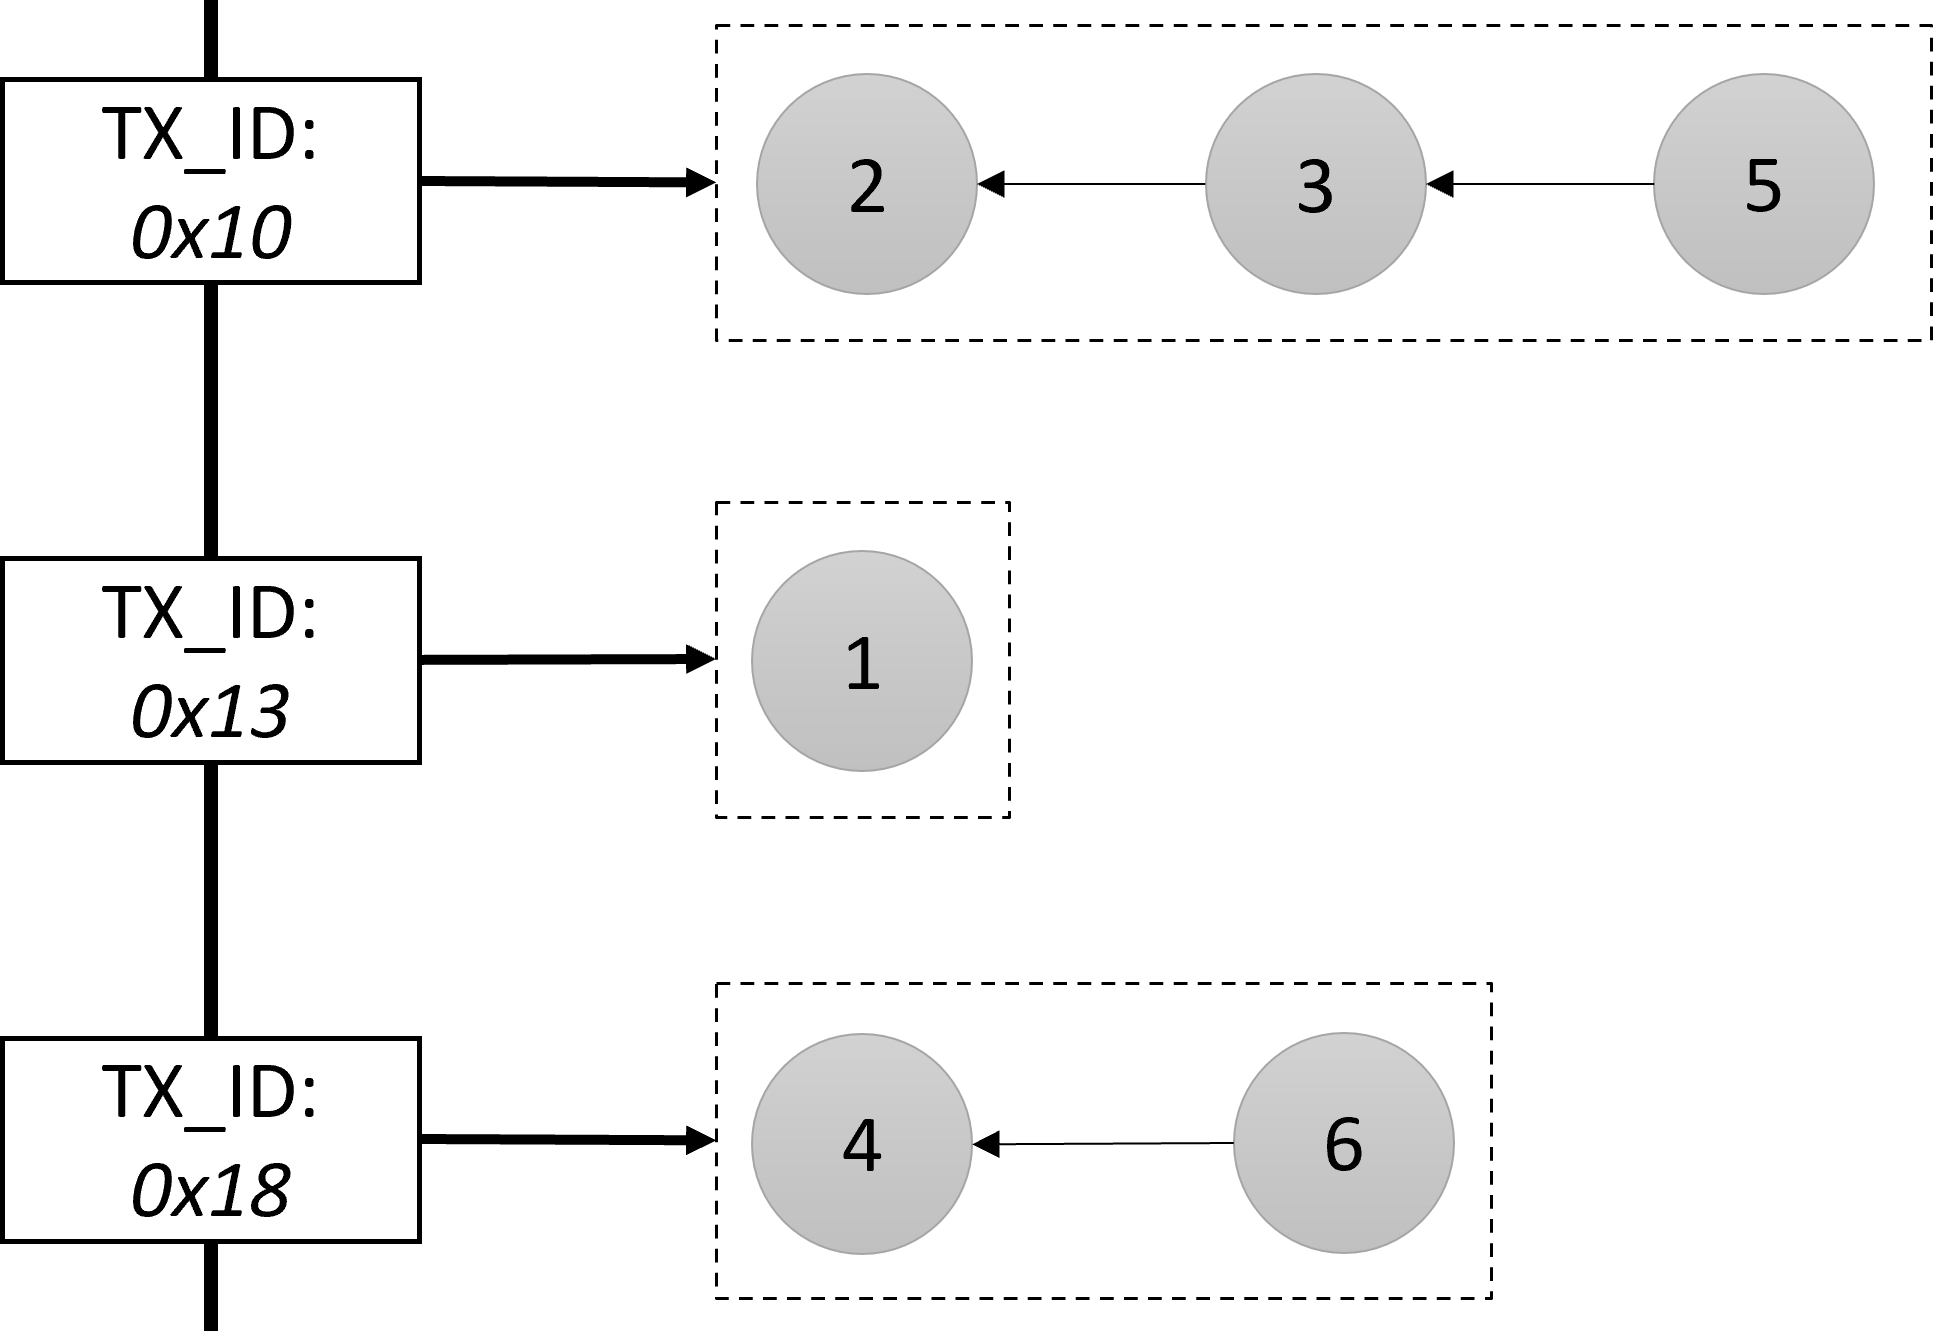
\includegraphics[width=0.7\textwidth]{Figures/store_comparision.png}
    \caption{Single DML PostgreSQL vs. Single HSQLDB}
    \label{fig:store_comparision}
\end{figure}


%%%%%%%%%%%%%%%%%%%%%%%%%%%%%%%%%%%%%%%%%%%%%%%%%%%%%%%%%%%%%%%%%%




\subsubsection{TERMINAL 1 vs TERMINAL 50 } 

Compare parallel worklaod. Use one terminal as a base set and the impact
it has on the overall performance.

\begin{figure}
    \centering
    \begin{subfigure}{.5\textwidth}
      \centering
      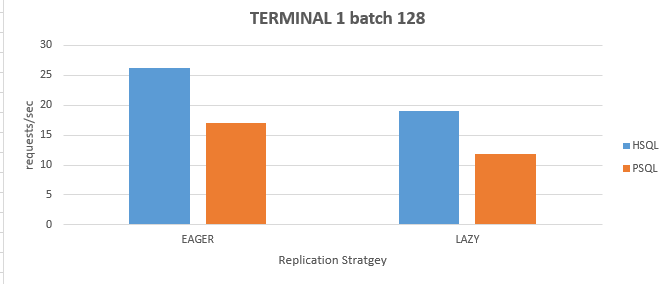
\includegraphics[width=.9\linewidth]{Figures/terminal1.PNG}
      \caption{One process}
      \label{fig:terminal1}
    \end{subfigure}%
    \begin{subfigure}{.5\textwidth}
      \centering
      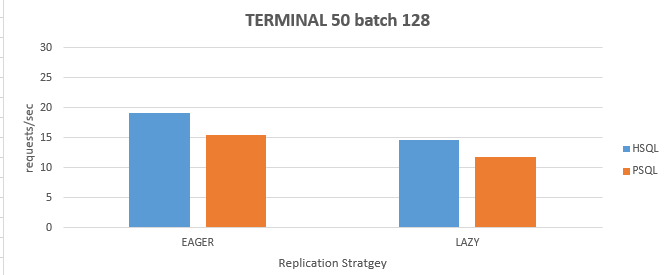
\includegraphics[width=.9\linewidth]{Figures/terminal50.PNG}
      \caption{50 processes}
      \label{fig:terminal50}
    \end{subfigure}
    \caption{Concurrency Comparison}
    \label{fig:terminal}
\end{figure}

Therefore from now on we will use TERMINAL 50 batch 128.

Show with equal stores lazy replicaiton is much smaller. Therefore also consider interlaving the stores and see which is faster in what area.
Which dowsnsides does it have

%%%%%%%%%%%%%%%%%%%%%%%%%%%%%%%%%%%%%%%%%%%%%%%%%%%%%%%%%%%%%%%%%%

\subsubsection{PSQL vs HSQL DML only} 
TERMINAL 50 batch 128
Compare Execution between PSQL and HSQL.
BOTH eager  -- PSQL EAGER HSQL LAZY -- HSQL EAGER PSQL --LAZY




\begin{figure}
    \centering
    \begin{minipage}{.5\textwidth}
      \centering
      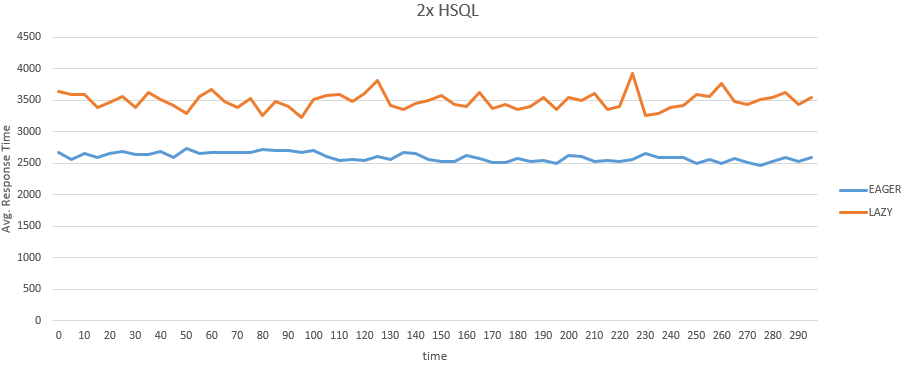
\includegraphics[width=.9\linewidth]{Figures/2hsql.PNG}
      \captionof{figure}{Avg. Latency of 2x HSQLDB. EAGER vs. LAZY}
      \label{fig:2hsql}
    \end{minipage}%
    \begin{minipage}{.5\textwidth}
      \centering
      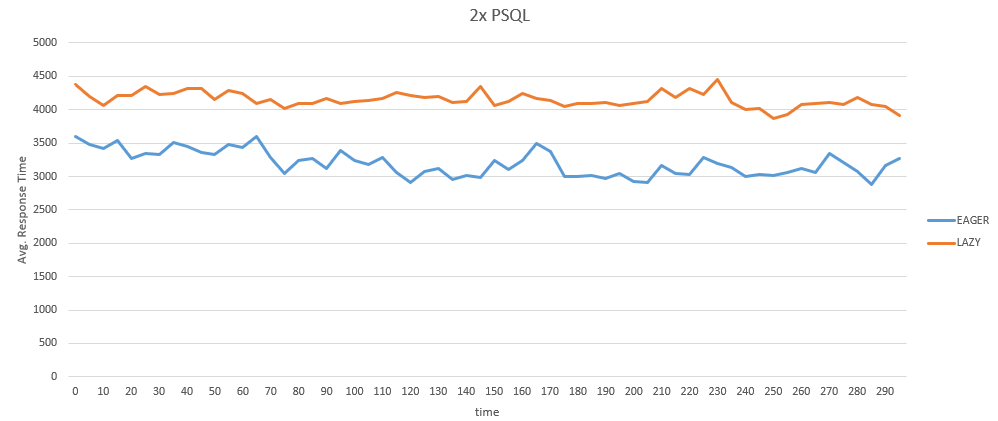
\includegraphics[width=.9\linewidth]{Figures/PSQL.PNG}
      \captionof{figure}{Avg. Latency of 2x PostgreSQL. EAGER vs. LAZY}
      \label{fig:2psql}
    \end{minipage}
    \end{figure}

Maybe combine teh four images
AVG HSQL 2x EAGER and LAZY
AVG PSQL 2x EAGER and LAZY
\todoMissing{Make the scale equal everywhere that to images are comparable}
\begin{figure}
    \centering
    \begin{minipage}{.5\textwidth}
      \centering
      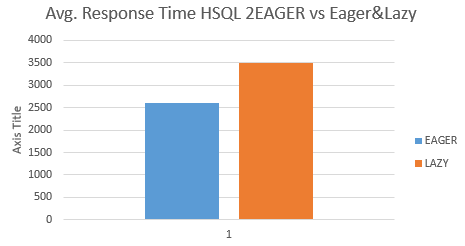
\includegraphics[width=.9\linewidth]{avg_response-hsql.PNG}
      \captionof{figure}{A figure}
      \label{fig:test1}
    \end{minipage}%
    \begin{minipage}{.5\textwidth}
      \centering
      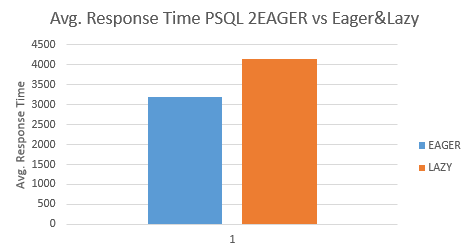
\includegraphics[width=.9\linewidth]{Figures/abg_response-psql.PNG}
      \captionof{figure}{Another figure}
      \label{fig:test2}
    \end{minipage}
    \end{figure}



DML onlyReponse time comparison HSQL and PSQL with switching stores
\begin{figure}[t] 
    \centering 
    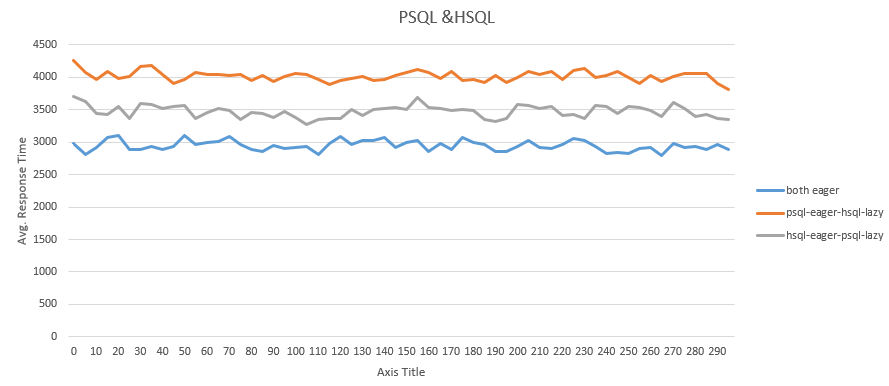
\includegraphics[width=0.7\textwidth]{Figures/PSQ_HSQL_DML_only.PNG}
    \caption{DML only - Avg. Latency comparsion PostgreSQL vs. HSQLDB. With switching Roles}
    \label{fig:psqlhsqlresponse}
\end{figure}



Identify that it makes a difference whihc store is eager and which one is lazy in terms of the  average respone time

Talk about and suspect why lazy replication is so much slower.
And identify that is is caused by the high and queue replication time
\begin{figure}[t] 
    \centering 
    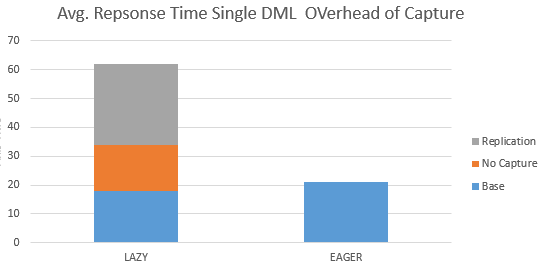
\includegraphics[width=0.7\textwidth]{Figures/dml_comp.PNG}
    \caption{Execution-Time comparision of a decompossed  single write-operation with and without data active data capture }
    \label{fig:write_decomposition}
\end{figure}

Therefore show how this deviates in General. What happens if we disable the replication queue or teh capture in geenral.
To immitate an on-demand processing where entities and placements are purposely kept at a given point

We see exactly the delay starting after 1 5se minute because afterwards the first placement could fulfil the freshness request and had to fallback to the primary who have might been locked
This graph exactly corresponds to the graph depicted in \ref{fig:write_decomposition} 
Mixed 60-40
\begin{figure}[t] 
    \centering 
    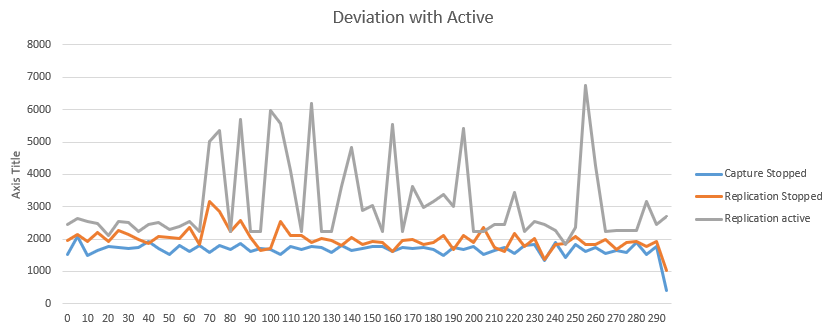
\includegraphics[width=0.7\textwidth]{Figures/deviation_with_active_que.PNG}
    \caption{Mixed Workload 60-40 with 100\% Freshness with relative read 1 minute }
    \label{fig:replication Impact}
\end{figure}



Even difference which of these stores is considered to be faster in priamry and faster as secondary

\begin{figure}
    \centering
    \begin{subfigure}{.5\textwidth}
      \centering
      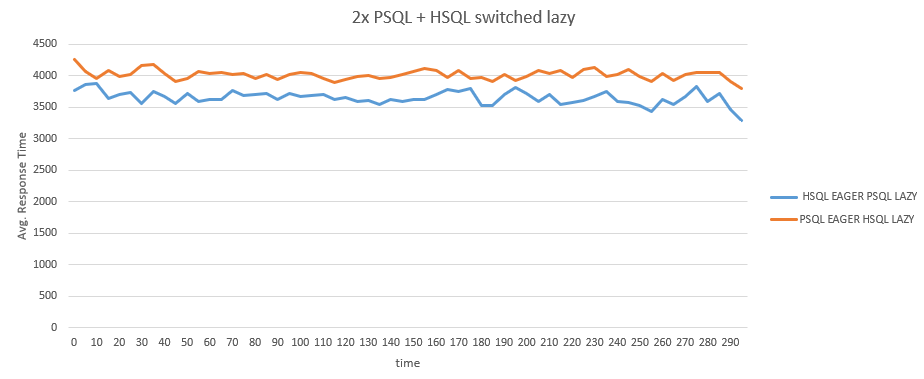
\includegraphics[width=.9\linewidth]{psql_hsql_switched_lazy.PNG}
      \caption{Comparison of 2 Stores HSQLDB and PostgreSQL. Switching Roles.}
      \label{fig:2store}
    \end{subfigure}%
    \begin{subfigure}{.5\textwidth}
      \centering
      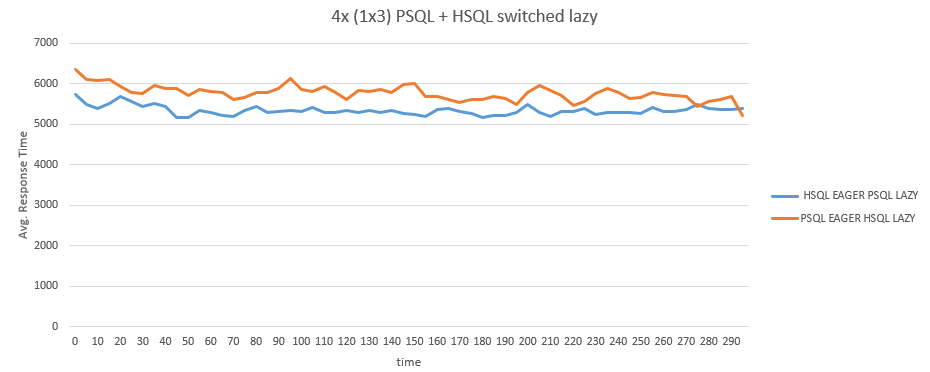
\includegraphics[width=.9\linewidth]{Figures/4psql_hsql_switched_lazy.PNG}
      \caption{Comparison of 4 Stores HSQLDB and PostgreSQL. Switching Roles.}
      \label{fig:4store}
    \end{subfigure}
    \caption{COmparison of different store sizes and swithcing Roles}
    \label{fig:24storecomp}
\end{figure}


\begin{figure}[t] 
    \centering 
    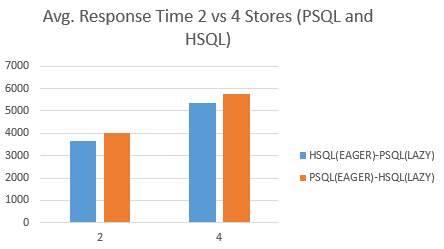
\includegraphics[width=0.7\textwidth]{Figures/24_avg_psql_hsql_switched_lazy.PNG}
    \caption{Avg. Response Time Comparison of different store sizes and swithcing Roles}
    \label{fig:}
\end{figure}



\begin{figure}[t] 
    \centering 
    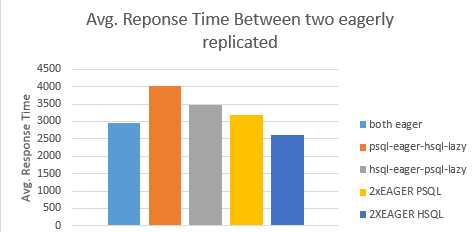
\includegraphics[width=0.7\textwidth]{Figures/psq_hsql_avg.response2.PNG}
    \caption{DML onlyAvg. Response Time Comparison of 2 store sizes and swithcing Roles}
    \label{fig:}
\end{figure}





%%%%%%%%%%%%%%%%%%%%%%%%%%%%%%%%%%%%%%%%%%%%%%%%%%%%%%%%%%%%%%%%%%


\subsubsection{Compare Total Replica Convergence Time DML only } 

BOTH eager  -- PSQL EAGER HSQL LAZY -- HSQL EAGER PSQL --LAZY
In terms of their execution and replication time which one finishes faster
Also does the numbe rof stores have an impact
Mixed Worklaod?

\begin{figure}[t] 
    \centering 
    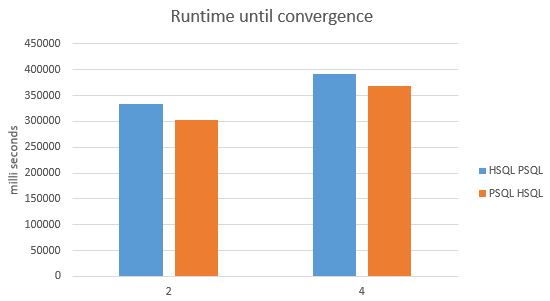
\includegraphics[width=0.7\textwidth]{Figures/runtime_convergence24.PNG}
    \caption{Convergence Time of PostgreSQL and HSQLDB with n-number of stores.}
    \label{fig:store_comparision}
\end{figure}


Average Repsonse Time accumulated with the Extension of teh Replicaiton Queue as well as the shrinking
to mimic the convergence time. 

\begin{figure}
    \centering
    \begin{minipage}{.5\textwidth}
      \centering
      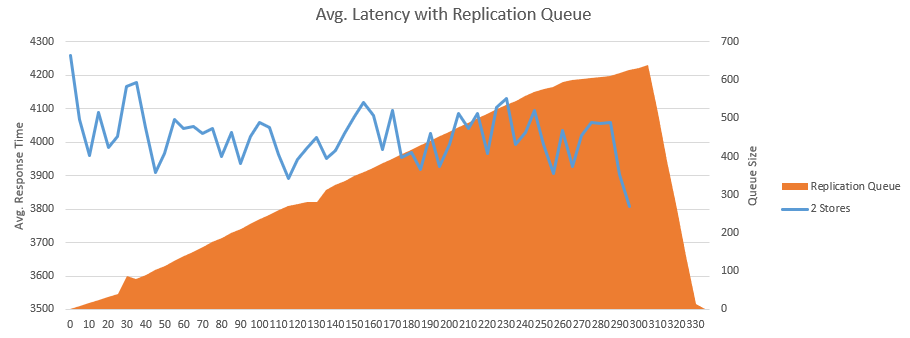
\includegraphics[width=.9\linewidth]{Figures/2latency_queue.PNG}
      \captionof{figure}{2 Stores Execution Time and Replication Convergence}
      \label{fig:converge_2}
    \end{minipage}%
    \begin{minipage}{.5\textwidth}
      \centering
      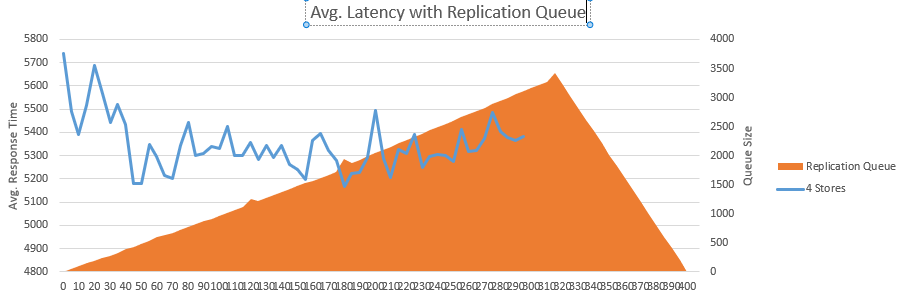
\includegraphics[width=.9\linewidth]{Figures/4latence_queue.PNG}
      \captionof{figure}{4 Stores Execution Time and Replication Convergence}
      \label{fig:converge_4}
    \end{minipage}
\end{figure}



\begin{figure}[t] 
    \centering 
    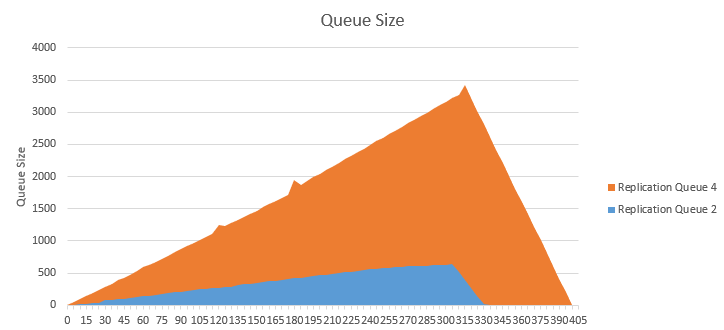
\includegraphics[width=0.7\textwidth]{Figures/queuesize24.PNG}
    \caption{Replication Queue Convergence}
    \label{fig:converge24}
\end{figure}
%%%%%%%%%%%%%%%%%%%%%%%%%%%%%%%%%%%%%%%%%%%%%%%%%%%%%%%%%%%%%%%%%%




\subsection*{Reponse Time DQL in General}

DQL only

No Freshness 
\begin{figure}[t] 
    \centering 
    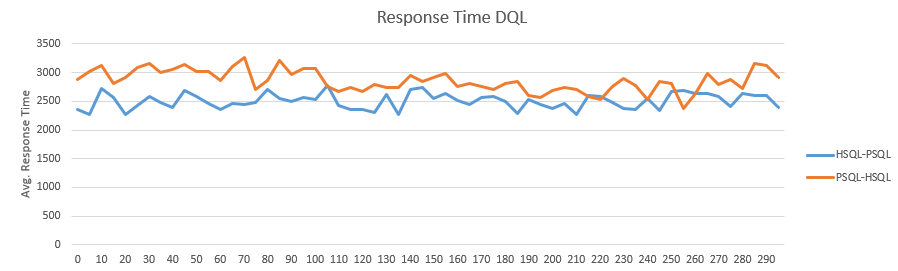
\includegraphics[width=0.7\textwidth]{Figures/psq_hsql_avg_response_no_fresh_dql.PNG}
    \caption{DQL No freshness}
    \label{fig:}
\end{figure}

\begin{figure}[t] 
    \centering 
    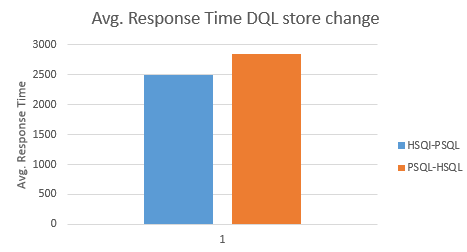
\includegraphics[width=0.7\textwidth]{avg_response-hsql-psql-dql_no_fresg.PNG}
    \caption{}
    \label{fig:}
\end{figure}




100 \% Freshness
\begin{figure}[t] 
    \centering 
    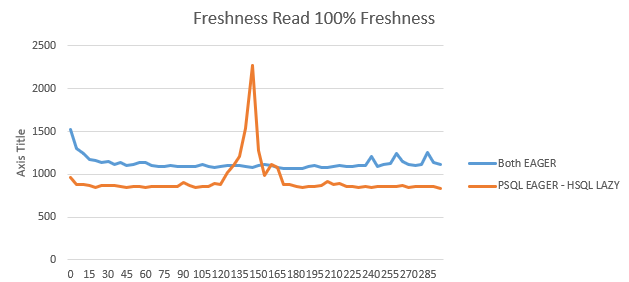
\includegraphics[width=0.7\textwidth]{Figures/100_fresh_dql.PNG}
    \caption{DQL 100\% Freshness }
    \label{fig:}
\end{figure}


DQL 50\% Freshness
\begin{figure}[t] 
    \centering 
    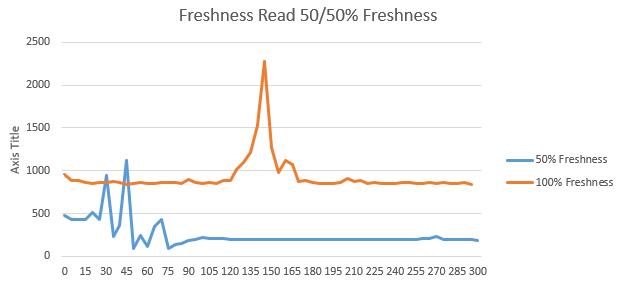
\includegraphics[width=0.7\textwidth]{Figures/50_fresh_dql.PNG}
    \caption{DQL 50\% Freshness}
    \label{fig:}
\end{figure}

%%%%%%%%%%%%%%%%%%%%%%%%%%%%%%%%%%%%%%%%%%%%%%%%%%%%%%%%%%%%%%%%%%

\subsubsection{Response Time impact on number of stores } 

Compare execution time with different number of stores 1 Eager n Lazy   (Because for Lazy there are more replications to put into the queue per pending operation)
\begin{figure}[t] 
    \centering 
    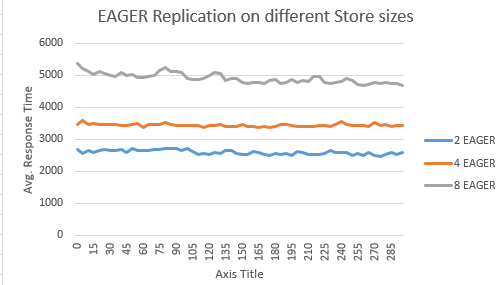
\includegraphics[width=0.7\textwidth]{Figures/hsql_eager_stores.PNG}
    \caption{}
    \label{fig:}
\end{figure}


\begin{figure}[t] 
    \centering 
    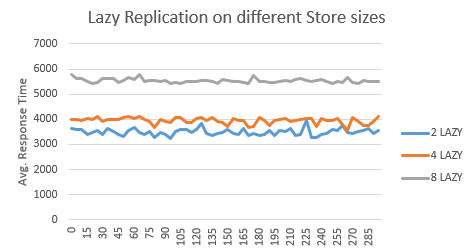
\includegraphics[width=0.7\textwidth]{Figures/hsql_lazy_stores.PNG}
    \caption{}
    \label{fig:}
\end{figure}


Stores in general stay rather stable how does this chaneg if 
Freshness impact if we have multiple partitions
\begin{figure}[t] 
    \centering 
    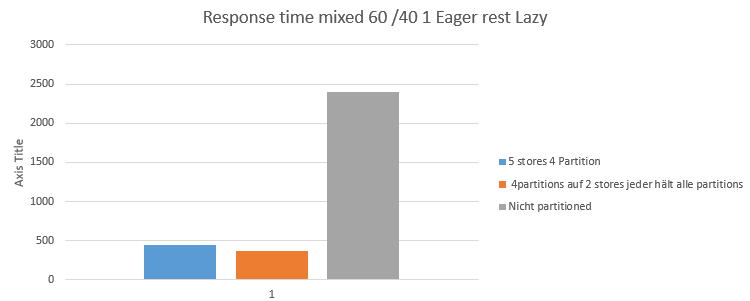
\includegraphics[width=0.7\textwidth]{Figures/partioned_freshness.PNG}
    \caption{}
    \label{fig:}
\end{figure}


Check the average repsonse Time
\begin{figure}[t] 
    \centering 
    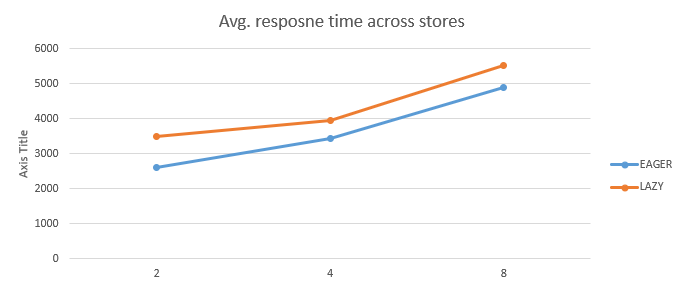
\includegraphics[width=0.7\textwidth]{Figures/hsql_avg_response_stores.PNG}
    \caption{}
    \label{fig:}
\end{figure}

%%%%%%%%%%%%%%%%%%%%%%%%%%%%%%%%%%%%%%%%%%%%%%%%%%%%%%%%%%%%%%%%%%

\subsubsection{Locking } 
\begin{figure}[t] 
    \centering 
    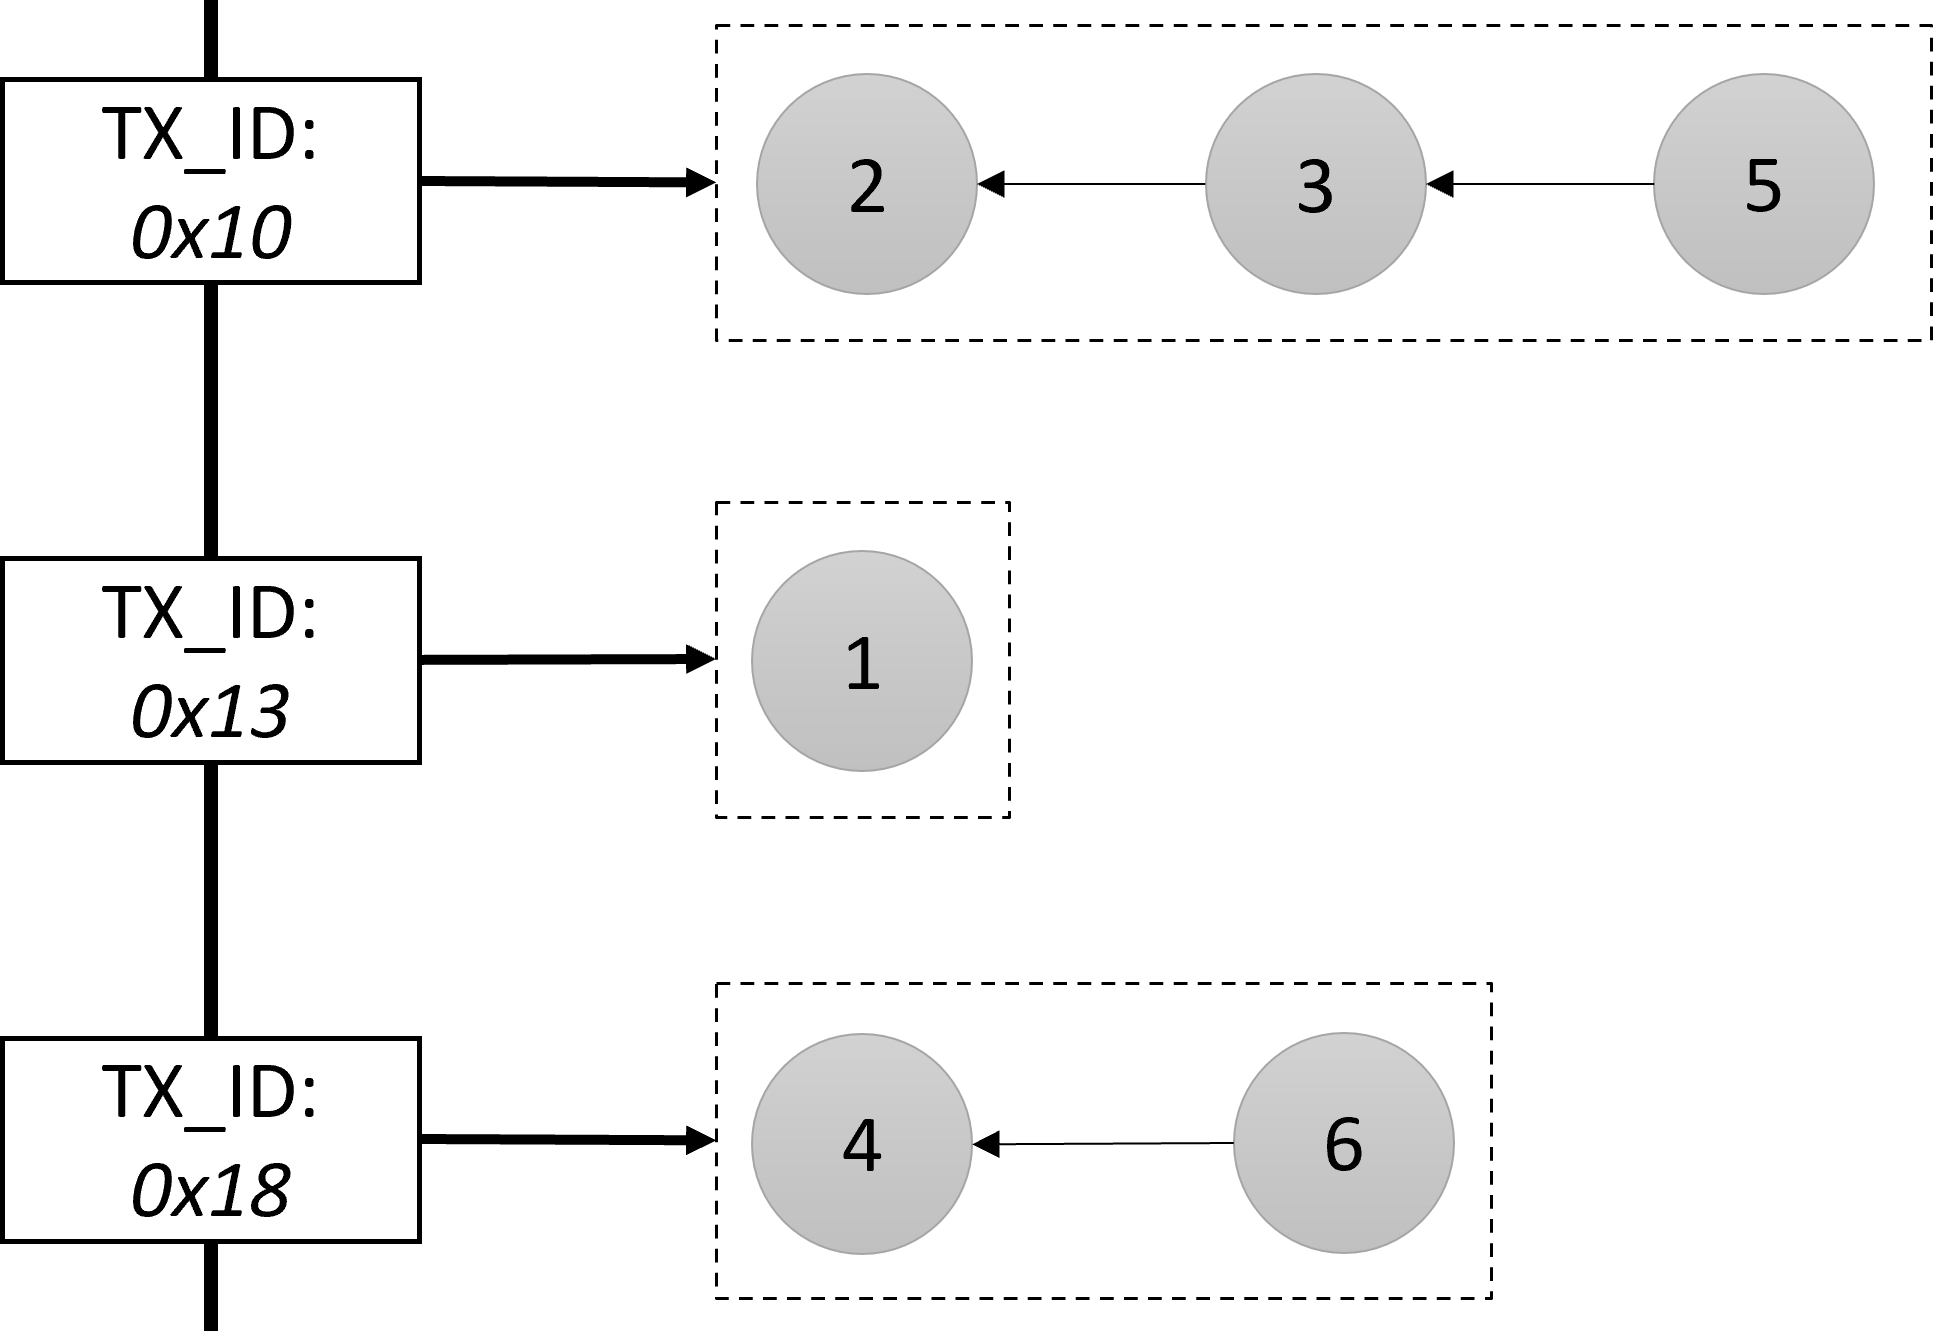
\includegraphics[width=0.7\textwidth]{Figures/store_comparision.png}
    \caption{}
    \label{fig:}
\end{figure}


%%%%%%%%%%%%%%%%%%%%%%%%%%%%%%%%%%%%%%%%%%%%%%%%%%%%%%%%%%%%%%%%%%
\subsubsection{Freshness Evaluation Type Filer} 
Show how each filter impacts the store differently, but all in all roughly the same
\begin{figure}[t] 
    \centering 
    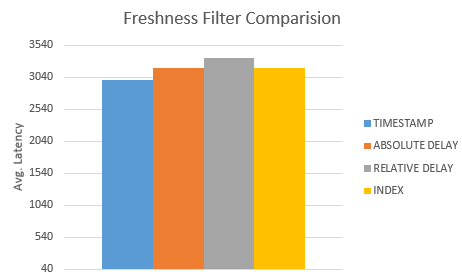
\includegraphics[width=0.7\textwidth]{Figures/freshness_comp.PNG}
    \caption{}
    \label{fig:}
\end{figure}


%%%%%%%%%%%%%%%%%%%%%%%%%%%%%%%%%%%%%%%%%%%%%%%%%%%%%%%%%%%%%%%%%%
\subsubsection{Mixed Worklaod} 

\begin{figure}[t] 
    \centering 
    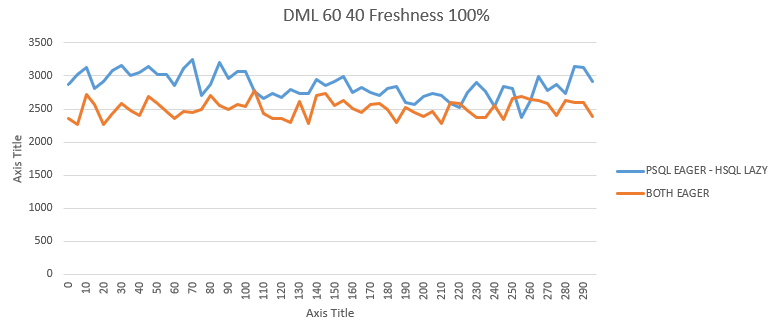
\includegraphics[width=0.7\textwidth]{Figures/60_40_fresh_100.PNG}
    \caption{60 R 40 W 100\% Freshness}
    \label{fig:}
\end{figure}




Show that the workload has a direct impact on the performance
\begin{figure}[t] 
    \centering 
    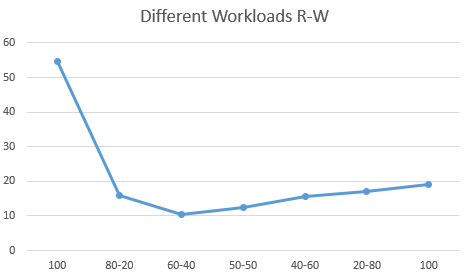
\includegraphics[width=0.7\textwidth]{Figures/different_ workloads.PNG}
    \caption{}
    \label{fig:}
\end{figure}

%%%%%%%%%%%%%%%%%%%%%%%%%%%%%%%%%%%%%%%%%%%%%%%%%%%%%%%%%%%%%%%%%%
%%%%%%%%%%%%%%%%%%%%%%%%%%%%%%%%%%%%%%%%%%%%%%%%%%%%%%%%%%%%%%%%%%
%%%%%%%%%%%%%%%%%%%%%%%%%%%%%%%%%%%%%%%%%%%%%%%%%%%%%%%%%%%%%%%%%%





\subsection{Results}
\label{sec:discussion}

The result generally shows
%%%%%%%%%%%%%%%%%%%%%%%%%%%%%%%%%%%%%%%%%%%%%%%%%%%%%%%%%%%%%%%%%%




